% !TeX spellcheck = ru_RU-Russian

\section{О регуляризации}

При решении задачи машинного обучения часто возникает проблема переобучения, при котором модель подстраивается под шум данных, что снижает ее обобщаю способность. 
Один из методов борьбы с этим --- регуляризации, или же сокращение весов (англ.: weight decay). Данный метод добавляет штраф к функции потерь за сложность модели, в случае линейных моделей~--- штраф за большие веса коэффициентов. Регуляризация ограничивает пространство решений и делает модель более устойчивой к шуму, что увеличивает вероятность корректных предсказаний на новых данных. Пример, когда усложнение модели, путем добавления избыточных коэффициентов полиномиальной модели представлен на рис.~\ref{liner-reg-overfitting}.

\begin{figure}[h]
	\centering
	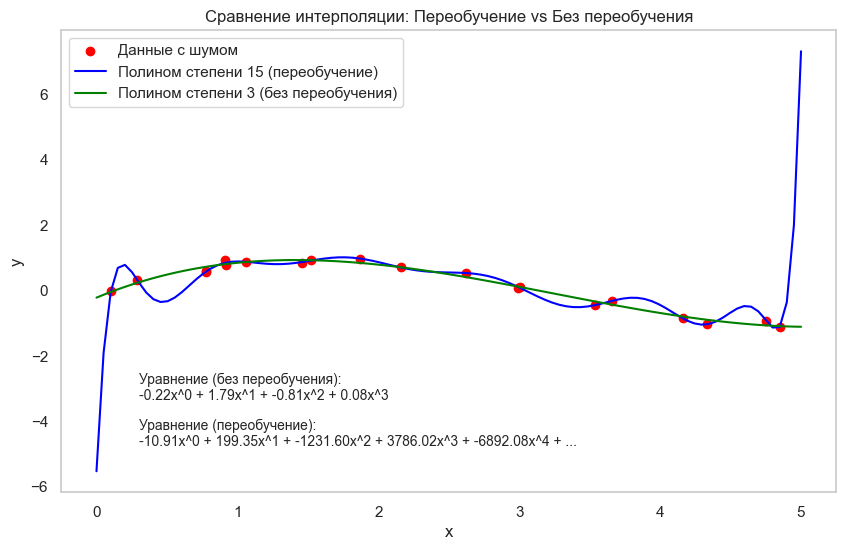
\includegraphics[width=0.9\linewidth]{chapters/linear/pics/reg-overfitting.png}
	\caption{Иллюстрация проблемы переобучения для решения линейной задачи}
	\label{linear-reg-overfitting}
\end{figure}

В разделе~\ref{linear-reg-l1l2} рассмотрены основные методы регуляризации, применяемые в линейных моделях. Раздел~\ref{linear-reg-prob} описывает вероятностную трактовку причин возникновения регуляризации. Завершается глава разделом~\ref{linear-reg-task}, который содержит три теоретических задачи по теме регрессии.

\subsection{Гауссовский и лапласовский регуляризаторы}
\label{linear-reg-l1l2}

Гауссовский и лапласовский регуляризаторы представляют собой две разные техники регуляризации, которые используются для управления сложностью моделей и предотвращения переобучения. Они основаны на различных подходах к штрафованию весов модели.

\subsubsection{Лапласовский регуляризатор (L1 регуляризатор)}

Лапласовский (L1) регуляризатор использует сумму модулей значений весов модели в качестве штрафа. Формально новую функцию потерь можно записать следующим образом:
$L1 = L_0 + \lambda \sum_{i=1}^{n} |w_i|$,
где $L_0$ --- исходная функция потерь, $|w_i|$ --- абсолютные значения весов модели, $\lambda$ --- коэффициент регуляризации.
\noindent
Преимущества:
\begin{itemize}
	\item Лапласовский регуляризатор может приводить к обнулению некоторых весов, что делает модель более интерпретируемой и позволяет выделять наиболее важные признаки.
	\item Он может быть особенно полезен в задачах с высокой размерностью, где много признаков могут быть неинформативными.
\end{itemize}
Недостатки:
\begin{itemize}
	\item Оптимизация с использованием L1 регуляризации может быть более сложной и требовать специальных алгоритмов (например, координатного спуска или методов, основанных на субградиенте).
\end{itemize}

\subsubsection{Гауссовский регуляризатор (L2 регуляризатор)}

Гауссовский (L2) регуляризатор использует штраф в виде суммы квадратов весов модели. Формально новую функцию потерь можно записать следующим образом:
$L2 = L_0 + \lambda \sum_{i=1}^{n} w_i^2$,
где $L_0$ — исходная функция потерь (например, среднеквадратичная ошибка для задачи регрессии), $w_i$ — веса модели, $\lambda$ — коэффициент регуляризации, который контролирует величину штрафа.
Преимущества:
\begin{itemize}
	\item Гауссовский регуляризатор помогает сгладить веса, что делает модель более устойчивой к шуму в данных.
	\item Он способствует распределению весов по всем признакам, уменьшая вероятность того, что некоторые признаки будут доминировать.
\end{itemize}
Недостатки:
\begin{itemize}
	\item Может не приводить к полному обнулению весов, поэтому не всегда приводит к интерпретируемым моделям.
\end{itemize}

\subsubsection {Сравнений L1 и L2 регуляризаторов}

Выбор между гауссовским и лапласовским регуляризаторами зависит от конкретной задачи и целей (сравнение см. в таблице~\ref{linear-reg-comp}). Если важна интерпретируемость модели и выделение значимых признаков, то стоит рассмотреть L1 регуляризацию. Если же цель — улучшить общее качество модели без сильного сокращения количества признаков, то L2 регуляризация может быть предпочтительнее. Это связано с тем, что в L2 регуляризации за счет возведения в квадрат значений весов вклад нулевого веса и просто малого веса неразличим на при наличии других выделенных признаков с весами порядка или более единицы. Таким образом, L2 регуляризация, в отличии от L1 не стремится обнулить коэффициенты, что снижает интерпретируемость модели. Однако квадратичная функция является гладкой, поэтому лучше поддается вычислительным методам оптимизации.

\begin{table}[h]
	\caption{Сравнение L1 и L2 регуляризаторов}
	\label{linear-reg-comp}
	\begin{tabular}{l|l|l}
		Характеристика & Лапласовский (L1) & Гауссовский (L2) \\
		\hline
		Штраф & Сумма абсолютных значений весов & Сумма квадратов весов \\
		Эффект на веса & Обнуление (спарсность) & Сглаживание \\
		Интерпретируемость & Выше & Меньше \\
		Оптимизация & Сложнее & Легче
	\end{tabular}
\end{table}

В ситуациях используется комбинация обоих методов регуляризации. Для этого вводится дополнительный гиперпараметр $\alpha$~--- доля первой нормы в штрафе за вес. Получается так называемая эластичная сеть (англ.: elastic net). В таком случае:
$L = L_0 + \lambda [\alpha \sum_{i=1}^{n} |w_i| + (1 - \alpha) \sum_{i=1}^{n} w_i^2]$. Данный подход позволяет учесть особенности двух подходов, однако усложняет модель.

\subsection {Вероятностная интерпретация регуляризации}
\label{linear-reg-prob}

В первом рассмотрении регуляризацию можно рассматриваться как введение априорной информации о параметрах модели. Рассмотрим вводимые предположения:
\begin{itemize}
	\item в случае L1 регуляризации мы предполагаем, что многие веса могут быть равны нулю, это соответствует идее о том, что истинная модель простая и присутствуют лишние признаки;
	\item в случае L2~--- веса распределены вблизи общего малого среднего значения, это отражает предположение о том, что все признаки вносят сопоставимый вклад в предсказание.
\end{itemize}
\noindent
Описанным выше предположениям о весах соответствуют экспоненциальное и нормальное распределения (см. рис.~\ref{linear-reg-distribution}). Рассмотрим их влияние на штраф и функцию потерь.

\begin{figure}[h]
	\centering
	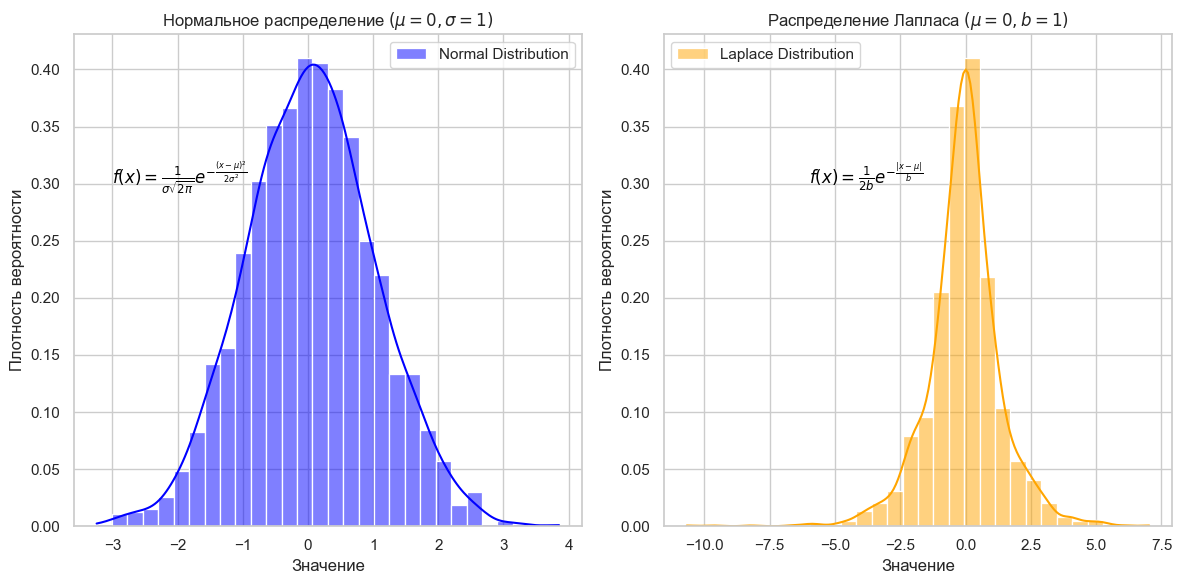
\includegraphics[width=0.9\linewidth]{chapters/linear/pics/reg-distributions.png}
	\caption{Сравнение экспоненциального и нормального распределений}
	\label{linear-reg-distribution}
\end{figure}

\subsubsection {L1 регуляризация}

предполагает, что веса $w_j$ распределены по лапласовскому закону (или двойному экспоненциальному распределению), $w_j - Laplace(0, b)$.

\subsubsection{L2 регуляризация} 

предполагает, что веса модели $w_j$ имеют нормальное распределение с нулевым средним и некоторой дисперсией $\sigma^2$. Это можно записать как $w_j - N(0, \sigma^2)$.

\subsection {Задачи}
\label{linear-reg-task}


\subsubsection{Вопрос 1}
\noindent Как изменение коэффициента $\lambda$ влияет на величину весов $w_j$?

\textbf{L1 регуляризация}

\noindent При увеличении $\lambda$ происходит обнулению некоторых весов $w_j$. Это приводит к тому, что с увеличением $\lambda$ количество ненулевых весов уменьшается, что может помочь в отборе признаков и упрощении модели.

\textbf{L2 регуляризация}

\noindent При увеличении $\lambda$ происходит увеличение штрафа за большие значения весов. Это приводит к уменьшению величины весов $w_j$ (все веса стремятся к нулю), что помогает избежать переобучения. В случае $\lambda$ = 0 модель не имеет регуляризации, и веса могут принимать любые значения, что может привести к переобучению.

\subsubsection{Вопрос 2}
\noindent Какова геометрическая интерпретация регуляризации в пространстве весов?

\begin{figure}[h]
	\centering
	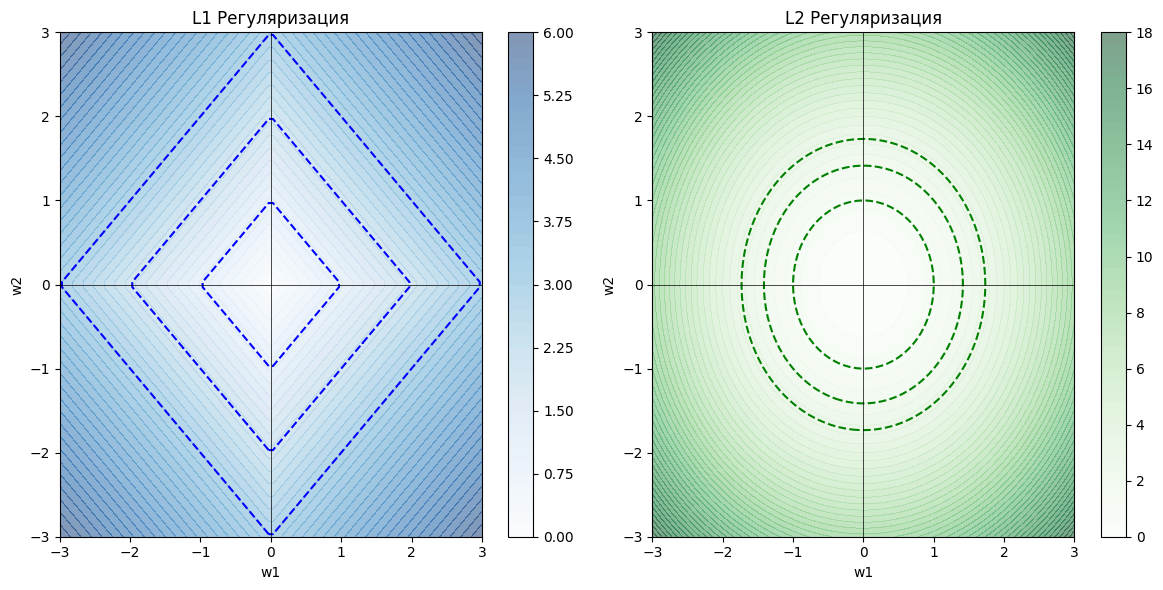
\includegraphics[width=0.9\linewidth]{chapters/linear/pics/reg-geom.png}
	\caption{Геометрическая интерпретация регуляризации в пространстве весов}
	\label{linear-reg-geom}
\end{figure}

\textbf{L1 регуляризация}

\noindent Геометрически L1 регуляризация создает ромбовидные (или параллелепипедные) области в пространстве весов. Оптимальные веса находятся на вершинах этих ромбов, что приводит к обнулению некоторых весов и, следовательно, к отбору признаков.

$L1(w_1,w_2) = const <=> |w_1|+|w_2| = const$

\textbf{L2 регуляризация}

\noindent Геометрически L2 регуляризация создает сферу (или гиперсферу) в пространстве весов, внутри которой минимизируется функция потерь. Это означает, что оптимальные веса будут находиться на поверхности этой сферы, что приводит к сглаживанию и уменьшению значений весов.

$L2(w_1,w_2) = const <=> w_1^2+w_2^2 = const$

\subsubsection{Вопрос 3}
\noindent Какие особенности признаков компенсируют регуляризации?

\textbf{L1 регуляризация}

\noindent Используя L1 регуляризацию, можно обнулить веса для менее значимых признаков. После обучения модели можно проанализировать ненулевые веса и оставить только те признаки, которые имеют значимые коэффициенты, тем самым осуществляя отбор признаков.

\textbf{L2 регуляризация}

\noindent L2 регуляризация помогает сгладить веса при наличии мультиколлинеарности, уменьшая их величину и тем самым снижая влияние коррелирующих признаков. Это позволяет избежать чрезмерного увеличения весов для сильно коррелирующих признаков.

\section*{Основная идея}

Градиентные методы --- это широкий класс оптимизационных алгоритмов, используемых не только в машинном обучении. Здесь градиентный подход будет рассмотрен в качестве способа подбора вектора синаптических весов \( w \) в линейном классификаторе. Пусть \( y^*: \, X \to Y \) — целевая зависимость, известная только на объектах обучающей выборки: \( X^l = (x_i, y_i)_{i=1}^l \), где \( y_i = y^*(x_i) \).

Найдём алгоритм \( a(x, w) \), аппроксимирующий зависимость \( y^* \). В случае линейного классификатора искомый алгоритм имеет вид:
$$ a(x, w) = \varphi\left(\sum_{j=1}^n w_j x^j - w_0\right), $$
где \( \varphi(z) \) играет роль функции активации (в простейшем случае можно положить \( \varphi(z) = \operatorname{sign}(z) \)).

Согласно принципу минимизации эмпирического риска, для этого достаточно решить оптимизационную задачу:
$$ Q(w) = \sum_{i=1}^l L(a(x_i, w), y_i) \to \min_w, $$
где \( L(a, y) \) — заданная функция потерь.

Для минимизации применим метод градиентного спуска (gradient descent). Это пошаговый алгоритм, на каждой итерации которого вектор \( w \) изменяется в направлении наибольшего убывания функционала \( Q \) (то есть в направлении антиградиента):
$$ w := w - \eta \nabla Q(w), $$
где \( \eta \) — положительный параметр, называемый темпом обучения (learning rate).

\subsection*{Основные подходы к реализации градиентного спуска}
\begin{enumerate}
    \item \textbf{Пакетный (batch):} на каждой итерации обучающая выборка просматривается целиком, и только после этого изменяется \( w \). Этот подход требует больших вычислительных затрат.
    \item \textbf{Стохастический (stochastic/online):} на каждой итерации из обучающей выборки случайным образом выбирается один объект. Таким образом, вектор \( w \) настраивается на каждый вновь выбираемый объект.
\end{enumerate}

\subsection*{Алгоритм Stochastic Gradient (SG)}
\textbf{Вход:}
\begin{itemize}
    \item \( X^l \) --- обучающая выборка;
    \item \( \eta \) --- темп обучения;
    \item \( \lambda \) --- параметр сглаживания функционала \( Q \).
\end{itemize}

\textbf{Выход:} Вектор весов \( w \)

\textbf{Тело алгоритма:}
\begin{enumerate}
    \item Инициализировать веса \( w_j \), \( j = 0, \dots, n \);
    \item Инициализировать текущую оценку функционала: \( Q := \sum_{i=1}^l L(a(x_i, w), y_i) \);
    \item Повторять:
    \begin{enumerate}
        \item выбрать объект \( x_i \) из \( X^l \) (например, случайным образом);
        \item вычислить выходное значение алгоритма \( a(x_i, w) \) и ошибку: \( \varepsilon_i := L(a(x_i, w), y_i) \);
        \item сделать шаг градиентного спуска:
        $$ w := w - \eta L_a^\prime (a(x_i, w), y_i) \varphi^\prime (\langle w, x_i \rangle)x_i; $$
        \item оценить значение функционала:
        $$ Q := (1 - \lambda)Q + \lambda\varepsilon_i; $$
    \end{enumerate}
    пока значение \( Q \) не стабилизируется и/или веса \( w \) не перестанут изменяться.
\end{enumerate}

\subsection*{Порядок выбора объектов}
В случае стохастического градиентного спуска объекты следует выбирать случайным образом, однако существуют эвристики, направленные на улучшение сходимости:
\begin{itemize}
    \item Перемешивание (shuffling): случайно выбирать объекты, попеременно из разных классов. Идея в том, что объекты из разных классов менее "похожи", чем объекты одного класса, поэтому вектор \( w \) будет сильнее изменяться.
    \item Можно выбирать объект с вероятностью, обратно пропорциональной величине ошибки на объекте. Следует учитывать, что такая эвристика делает метод чувствительным к шумам.
\end{itemize}

\subsection*{Способы инициализации весов}
\begin{enumerate}
    \item Инициализация вектора \( w \) нулями.
    \item \( w_j := \operatorname{rand}\left(-\frac{1}{n}, \frac{1}{n}\right) \), где \( n \) — размерность пространства признаков.
    \item Решение исходной оптимизационной задачи при условии статистически независимых признаков, линейной функции активации (\( \varphi \)) и квадратичной функции потерь (\( L \)):
    $$ w_j := \frac{\langle y, f_j \rangle}{\langle f_j, f_j \rangle}. $$
\end{enumerate}

\subsection*{Параметр сглаживания}
Для оценки функционала \( Q \) на каждой итерации используется его приближённое значение по методу экспоненциального сглаживания, откуда \( \lambda \) лучше брать порядка \( \frac{1}{l} \).

\subsection*{Известные частные случаи алгоритма}
Метод SG (при соответствующем выборе функций активации и потерь) является обобщением следующих эвристик подбора \( w \) и алгоритмов классификации:
\begin{itemize}
    \item Адаптивный линейный элемент (Adalines);
    \item Правило Хэбба;
    \item Алгоритм \( k \)-средних (K-Means);
    \item Learning Vector Quantization (LVQ).
\end{itemize}

\subsection*{Преимущества SG}
\begin{itemize}
    \item Метод подходит для динамического (online) обучения.
    \item Алгоритм способен обучаться на избыточно больших выборках.
    \item Различные стратегии обучения позволяют адаптировать алгоритм для задач с избыточной или небольшой выборкой.
\end{itemize}

\subsection*{Недостатки SG и способы их устранения}
\begin{itemize}
    \item Возможны проблемы сходимости. Для борьбы с этим применяют технику встряхивания коэффициентов.
    \item При высокой размерности пространства признаков \( n \) и/или малой длине выборки \( l \) возможно переобучение. Для борьбы с этим применяют метод сокращения весов:
    $$ Q_{\tau}(w) = Q(w) + \frac{\tau}{2}||w||^2. $$
    Тогда правило обновления весов принимает вид:
    $$ w := w(1 - \eta \tau) - \eta \nabla Q(w). $$
    \item При больших значениях \( \langle w, x_i \rangle \) значение \( \varphi^\prime \) может становиться близким к нулю. Для предотвращения этого состояния вводят нормализацию признаков:
    $$ x^j := \frac{x^j - x_{\min}^j}{x_{\max}^j - x_{\min}^j}, \quad j = 1, \dots, n, $$
    где \( x_{\min}^j, x_{\max}^j \) — минимальное и максимальное значения признака \( j \)-го признака. Регуляризация, такая как weight decay, также помогает избежать "паралича".
\end{itemize}

\subsection*{Сходимость алгоритма}
Сходимость гарантируется при выпуклой функции \( Q(w) \) и выполнении следующих условий:
$$ \eta_t \xrightarrow{t \to \infty} 0, \quad \sum_{t=1}^{\infty} \eta_t = \infty, \quad \sum_{t=1}^{\infty} \eta_t^2 < \infty. $$
Например, можно положить \( \eta_t = \frac{\eta_0}{t} \), хотя на практике это не всегда удачно.

\section*{Задачи}

\subsection*{Задача 1: Доказать сходимость алгоритма при условиях выше}

\textbf{Решение:}

\begin{enumerate}
    \item \textbf{Выпуклость функции:} Поскольку \( Q(w) \) выпукла, мы можем использовать свойства выпуклых функций. Для любого \( w \) и \( w^* \) (где \( w^* \) — точка минимума функции \( Q \)) выполняется неравенство:
    $$ Q(w) \geq Q(w^*) + \nabla Q(w^*)^T (w - w^*). $$

    \item \textbf{Итерация метода стохастического градиента:} Обновление весов в SGD задается следующим образом:
    $$ w_{t+1} = w_t - \eta_t \nabla Q(w_t; \xi_t), $$
    где \( \xi_t \) — случайная переменная, представляющая выборку данных на итерации \( t \).

    \item \textbf{Анализ изменения функции:} Мы можем оценить изменение функции \( Q \) на каждой итерации:
    $$ Q(w_{t+1}) \leq Q(w_t) + \nabla Q(w_t; \xi_t)^T (w_{t+1} - w_t) + \frac{L}{2} \|w_{t+1} - w_t\|^2, $$
    где \( L \) — константа Липшица для градиента \( \nabla Q \).

    Подставляя обновление:
    $$ Q(w_{t+1}) \leq Q(w_t) - \eta_t \nabla Q(w_t; \xi_t)^T \nabla Q(w_t) + \frac{L}{2} \eta_t^2 \|\nabla Q(w_t; \xi_t)\|^2. $$

    \item \textbf{Суммирование изменений:} Суммируя по всем итерациям, мы получаем:
    $$ \sum_{t=1}^{T} Q(w_{t+1}) - Q(w_1) \leq -\sum_{t=1}^{T} \eta_t \nabla Q(w_t; \xi_t)^T \nabla Q(w_t) + \sum_{t=1}^{T} \frac{L}{2} \eta_t^2 \|\nabla Q(w_t; \xi_t)\|^2. $$

    \item \textbf{Использование условий:} Условия \( \sum_{t=1}^{\infty} \eta_t = \infty \) и \( \sum_{t=1}^{\infty} \eta_t^2 < \infty \) позволяют нам сделать вывод о том, что:
    \begin{itemize}
        \item Сумма шагов обучения стремится к бесконечности, что означает, что веса \( w_t \) будут продолжать обновляться.
        \item Сумма квадратов шагов обучения конечна, что позволяет контролировать величину изменений на каждой итерации.
    \end{itemize}

    \item \textbf{Сходимость к минимуму:} В результате, при условии, что \( Q(w) \) выпукла, и учитывая условия на шаги обучения, мы можем утверждать, что последовательность \( w_t \) будет сходиться к некоторой точке \( w^* \), которая является минимумом функции \( Q(w) \).
\end{enumerate}

Таким образом, метод стохастического градиента сходится к минимуму выпуклой функции \( Q(w) \) при выполнении заданных условий.

\subsection*{Задача 2: Оценка вариации градиента}

\textbf{Условие:} Пусть \( \xi_1, \xi_2, \ldots, \xi_n \) — независимые и одинаково распределённые (i.i.d.) случайные переменные, представляющие собой выборки из обучающего набора. Рассмотрим стохастический градиент \( \nabla L(\theta; \xi_t) \).

\textbf{Задача:} Доказать, что математическое ожидание стохастического градиента совпадает с истинным градиентом функции потерь:
\[
\mathbb{E}[\nabla L(\theta; \xi_t)] = \nabla L(\theta)
\]
и оценить дисперсию \( \operatorname{Var}(\nabla L(\theta; \xi_t)) \) в зависимости от размера выборки \( n \).

\subsection*{Доказательство}

\begin{enumerate}
    \item \textbf{Определение стохастического градиента:} Пусть \( L(\theta) \) — функция потерь, зависящая от параметров \( \theta \) и от выборки \( \xi \). Мы можем записать функцию потерь как среднее значение по всем данным:
    $$ L(\theta) = \frac{1}{n} \sum_{i=1}^{n} l(\theta; x_i, y_i), $$
    где \( l(\theta; x_i, y_i) \) — функция потерь для примера \( (x_i, y_i) \).

    \item \textbf{Истинный градиент:} Тогда истинный градиент функции потерь можно выразить как:
    $$ \nabla L(\theta) = \frac{1}{n} \sum_{i=1}^{n} \nabla l(\theta; x_i, y_i). $$

    \item \textbf{Математическое ожидание стохастического градиента:} Теперь рассмотрим стохастический градиент:
    $$ \nabla L(\theta; \xi_t) = \nabla l(\theta; \xi_t), $$
    где \( \xi_t \) — случайная выборка. Поскольку \( \xi_t \) выбирается из одного из \( n \) примеров, математическое ожидание стохастического градиента будет:
    \[
    \mathbb{E}[\nabla L(\theta; \xi_t)] = \mathbb{E}[\nabla l(\theta; \xi_t)] = \frac{1}{n} \sum_{i=1}^{n} \nabla l(\theta; x_i, y_i) = \nabla L(\theta).
    \]
    Таким образом, мы доказали, что:
    \[
    \mathbb{E}[\nabla L(\theta; \xi_t)] = \nabla L(\theta).
    \]

    \item \textbf{Оценка дисперсии:} Теперь найдём дисперсию стохастического градиента:
    \[
    \operatorname{Var}(\nabla L(\theta; \xi_t)) = \mathbb{E}[(\nabla L(\theta; \xi_t) - \mathbb{E}[\nabla L(\theta; \xi_t)])^2].
    \]
    Подставим выражение для стохастического градиента:
    \[
    \operatorname{Var}(\nabla L(\theta; \xi_t)) = \mathbb{E}[(\nabla l(\theta; \xi_t) - \nabla L(\theta))^2].
    \]
    Поскольку \( \xi_t \) является случайным выбором, мы можем использовать свойства дисперсии. Для \( n \) независимых и одинаково распределённых (i.i.d.) выборок дисперсия стохастического градиента будет уменьшаться с увеличением размера выборки:
    $$ \operatorname{Var}(\nabla L(\theta; \xi_t)) = \frac{1}{n} \operatorname{Var}(l(\theta; x, y)), $$
    где \( (x, y) \) — случайная выборка из обучающего набора. Это означает, что дисперсия стохастического градиента уменьшается с увеличением размера выборки \( n \).
\end{enumerate}

\subsection*{Задача 3: Регуляризация и стохастический градиент}

\subsection*{Условие}
Рассмотрим функцию потерь с L2-регуляризацией:
$$ L(\theta) = \frac{1}{n} \sum_{i=1}^{n} l(\theta; x_i, y_i) + \frac{\lambda}{2} \|\theta\|^2 $$
где \( l(\theta; x_i, y_i) \) — функция потерь для примера \( (x_i, y_i) \), а \( \lambda \) — коэффициент регуляризации.

\subsection*{Задача}
Обосновать, как регуляризация влияет на сходимость метода стохастического градиента, и показать, что использование регуляризации может помочь избежать переобучения, уменьшая значение функции потерь на валидационном наборе.

\subsection*{Влияние регуляризации на сходимость метода стохастического градиента}
\begin{enumerate}
    \item \textbf{Сглаживание функции потерь:}
    \begin{itemize}
        \item Добавление L2-регуляризации к функции потерь делает её более гладкой и выпуклой. Это связано с тем, что регуляризационный член \( \frac{\lambda}{2} \|\theta\|^2 \) добавляет "наказание" за большие значения параметров, что предотвращает резкие изменения градиента.
        \item Гладкость функции потерь способствует более стабильному обновлению параметров при использовании стохастического градиента. Это означает, что обновления параметров будут более предсказуемыми и менее подвержены шуму, что улучшает сходимость алгоритма.
    \end{itemize}

    \item \textbf{Уменьшение переобучения:}
    \begin{itemize}
        \item Регуляризация способствует уменьшению значений параметров модели, что, в свою очередь, снижает сложность модели. Это позволяет избежать переобучения, когда модель слишком точно подстраивается под тренировочные данные, включая шум.
        \item В результате, при использовании регуляризации, модель будет лучше обобщаться на новых данных, что выражается в меньшем значении функции потерь на валидационном наборе.
    \end{itemize}
\end{enumerate}

\subsection*{Доказательство эффекта регуляризации на валидационном наборе}
\begin{enumerate}
    \item \textbf{Функция потерь на валидационном наборе:}
    \begin{itemize}
        \item Пусть \( L_{val}(\theta) \) — функция потерь на валидационном наборе. При использовании регуляризации, мы можем записать:
        $$ L_{val}(\theta) = \frac{1}{m} \sum_{j=1}^{m} l(\theta; x_j, y_j) + \frac{\lambda}{2} \|\theta\|^2 $$
        где \( m \) — количество примеров в валидационном наборе.
    \end{itemize}

    \item \textbf{Сравнение значений функции потерь:}
    \begin{itemize}
        \item Без регуляризации, модель может иметь высокую функцию потерь на валидационном наборе из-за переобучения. При добавлении L2-регуляризации, даже если функция потерь на тренировочном наборе остаётся низкой, регуляризация помогает поддерживать значение функции потерь на валидационном наборе на более низком уровне.
    \end{itemize}

    \item \textbf{Кросс-валидация для выбора \( \lambda \):}
    \begin{itemize}
        \item Оптимальное значение \( \lambda \) можно выбрать с помощью кросс-валидации. Это позволяет находить компромисс между сложностью модели и её обобщающей способностью, что в конечном итоге приводит к меньшему значению функции потерь на валидационном наборе.
    \end{itemize}
\end{enumerate}

\subsection*{Заключение по задаче 3}
Регуляризация, особенно L2-регуляризация, играет ключевую роль в улучшении сходимости метода стохастического градиента и в предотвращении переобучения модели. Она помогает сделать функцию потерь более гладкой и выпуклой, что способствует стабильности обновлений параметров. В результате, использование регуляризации приводит к лучшему обобщению модели и снижению значения функции потерь на валидационном наборе, что является важным аспектом при разработке надёжных моделей в машинном обучении.